%% -*- coding: utf-8; -*-

% Use 'digital' option to enable back references. This option is recommended for digital pdf version
%\documentclass[phd,american,digital]{thesispuc}%english thesis
%\documentclass[mscr,american]{thesispuc}%english dissertation
%\documentclass[phd,brazilian]{thesispuc}%tese em portugês
\documentclass[msc,brazilian]{thesispuc}%disseretação em portuguŝ


%%%
%%% Additional Packages
%%%
\usepackage{tabularx}
\usepackage{multirow}
\usepackage{multicol}
\usepackage{colortbl}
\usepackage[%
    dvipsnames,
    svgnames,
    x11names,
    fixpdftex,
    table
]{xcolor}
\usepackage{numprint}
\usepackage{textcomp}
\usepackage{booktabs}
\usepackage{amsmath}
\usepackage{enumitem}
\usepackage{amssymb}
\usepackage{svg}
% ABNT reference style package. The current style is the alphabetical order, if you need
% change to citation order, change in the line above 'alf' to 'num', also at the end replace
% bibliographystyle with the commented version.
\usepackage[num]{abntex2cite}
%\usepackage{tikz}
%\usepackage[linesnumbered, ruled, vlined]{algorithm2e}
%\usepackage{pgfplots,pgfplotstable} 
%\usepackage{array}
\usepackage{longtable}


%% numprint 
\npthousandsep{.}
\npdecimalsign{,}

%% ThesisPUC option
%\tablesmode{fig} %% [nada, fig, tab ou figtab]
%\algoritmsmode{none} %% [none ou use] %% Default is [use]
%\codesmode{none} %% [none ou use] %% Default is [use]
%\abreviationsmode{none} %% [none ou use] %% Default is [use]

\tablesmode{figtab}

\algorithmsmode{none}
\codesmode{none}
\abreviationsmode{use}

% \makeatletter  \renewcommand\@biblabel[1]{#1}  \makeatother

%%%
%%% Counters
%%%

%% uncomment and change for other depth values
\setcounter{tocdepth}{1}
%\setcounter{lofdepth}{3}
%\setcounter{lotdepth}{3}
%\setcounter{secnumdepth}{3}

%%%
%%% Misc.
%%%

\usecolour{true}
%% \graphicspath{ {./figuras/} }
%% https://www.overleaf.com/learn/latex/Inserting_Images
\citebrackets[]

\renewcommand{\arraystretch}{1.5}


%%%
%%% Titulos
%%%

\tituloglossario{Lista de Abreviaturas}
\autor{Antenor Moreira de Barros Leal}
\autorR{Leal, Antenor Moreira de Barros}

\advisor{Adriano Francisco Branco}{Prof.}
\advisorR{Branco, Adriano Francisco}
% If the advisor's department is different from author's department, uncomment the next line and type the correct name and acronym of advisor's institution.
%\advisorInst{institution name}{acronym}

%\coadvisor{Otávio da Fonseca Martins Gomes}{Dr.}
%\coadvisorR{da Fonseca Martins Gomes, Otávio}
%\coadvisorInst{Centro de Tecnologia Mineral}{CETEM/MCTI}

\title{Aplicativo web de auxílio à navegação aérea}
\titleuk{Aerial navigation aid web application}

%%\subtitulo{Aqui vai o subtitulo caso precise}

\day{16}
\month{Junho}
\year{2024}

\city{Rio de Janeiro}
\CDD{004} 
\department{Informática}
\program{\mbox{Engenharia} da \mbox{Computação}}
\school{\mbox{Engenharia} da \mbox{Computação}}
\university{Pontifícia Universidade Católica do Rio de Janeiro}
\uni{PUC-Rio}


%%%
%%% Jury
%%%

\jury{%
  \jurymember{xxxxxxxxxxxxxxxx}{Prof.}
    {Departamento de Informática}{PUC-Rio}
  \jurymember{xxxxxxxxxxxxxxx}{Prof.}
    {Departamento de Informática}{PUC-Rio}
   \jurymember{xxxxxxxxxxxxxxx}{Prof.}
    {Departamento de Informática}{PUC-Rio}
}


%%%
%%% Personal Resume
%%%

\resume{%
% If it fit in one line use this command:
\makebox[\textwidth][s]{Graduando em Engenharia da Computação na PUC - Rio}%
% If not just type your resume without any special command 
}


%%%
%%% Catalog prekeywords
%%%

\catalogprekeywords{%
  \catalogprekey{Informática}%
}

%%%
%%% Keywords - Don't use % at the end of /key dfinition
%%%

\keywords{%
    \key{Aviação}
    \key{Navegação}
    \key{Aplicativo}
    \key{Algoritmo}
    \key{Web}
    \key{Internet}
}

\keywordsuk{%
    \key{Aviation}
    \key{Navigation}
    \key{Application}
    \key{Algoritm}
    \key{Web}
    \key{Internet}
}


%%%
%%% Abstract
%%%

\abstract{%
É um aplicativo web de código aberto com o objetivo de auxiliar usuários de simuladores de voo que não possuem
acesso à ferramenta (Electronic Flight Bag) que um piloto de linha aérea teria. Ao acessar o aplicativo, o usuário
se depara com a lista de aeroportos cadastrados e, após escolher um, são exibidas as informações da pista,
frequências do aeroporto (torre, solo, ATIS, etc.), e frequências de navegação (ILS, VOR, etc.). Também são
apresentadas as informações das condições meteorológicas atuais do aeródromo (vento, visibilidade,
temperatura, etc.), tanto no formato oficial (\abrev METAR), obtidas a cada hora de uma API externa, como em um texto
em linguagem natural para melhor entendimento do jogador iniciante. Um usuário com permissão de
administrador pode adicionar e editar aeroportos. Módulos adicionais estão disponíveis como o cálculo da pista
em uso (a partir de informações do vento) e do perfil de descida.
} 

\abstractuk{%
It is an open source web application to auxialiate the flight simulator's users that don't have
access to the tool (Electronic Flight Bag) that an airline pilot would have. When accessing the app, the users
encounter the list of registered airports and, after choosing one, runway information, airport frequencies 
(tower, ground, ATIS etc) and navigation frequencies (ILS, VOR etc) are showed. Also provided are the current 
meteorological conditions of the aerodrome (wind, visibility, temperature, etc.), both in the official 
format (METAR), obtained hourly from an external API, and in natural language text for better 
understanding by novice players. An administrator user can add and edit airports. Based on the 
current wind information, the active runway is calculated. Additional modules are available such as calculation 
of the runway in use (from wind information) and the descent profile.
}


%%%
%%% Dedication
%%%

% xxxxxxxxxxxxxxxxxxxxxxxx Dedicatória aqui xxxxxxxxxxxxxxxxxxxxxxx
\dedication{%
  
}

%%%
%%% Epigraph
%%%

% epígrafe xxxxxxxxxxxxxxxx
\epigraph{%
 
}
\epigraphauthor{ }
\epigraphbook{ }

%--------------------------------------------
% \usepackage{draftwatermark}

% \SetWatermarkText{{\normalfont SEGUNDA ENTREGA (26/06) rev 1}}

% \SetWatermarkScale{0.2}
% \SetWatermarkAngle{0}
% \SetWatermarkColor{red!80!white}
% \SetWatermarkHorCenter{0.5\paperwidth}
% \SetWatermarkVerCenter{0.1\paperheight}
%--------------------------------------------


\begin{document}
  \chapter{Introdução}

xxxxxxxxxxxxxxxxxxxxxxxxxxxxxxxxxxxxxxx
  % Revisão OK 25/09
\chapter{Sistemas Similares}
Os EFBs possuem funções variadas como cálculo de combustível, gasto de combustível
em voo, velocidades de decolagem, etc. \cite{wired-efb} Para aeronaves mais novas, como o Airbus 
A320neo (New Engine Option), é difícil implementar o cálculo de performance e combustível, pois não 
é disponibilizado ao público como este cálculo é feito. Ferramentas encontradas 
na Internet \cite{a320-perf}, normalmente usan engenharia reversa, e, portanto, 
podem apresentar resultados diferentes de um cálculo oficial feito no aplicativo
de tablet.

Nos simuladores de voo para computador pessoal, algumas aeronaves simulam
este equipamento como o Airbus A320neo desenvolvido pela \textit{FlyByWire Simulations}. 
Apesar de ser uma aeronave \textit{freeware}, ela é bem sofisticada, chegando ao 
nível de realismo da \textit{Fenix Simulations} ou da \textit{ToLiss Simulations}, 
duas produtoras com modelos pagos do A320.

\begin{figure}%
    \centering
    \subfloat[\centering EFB no Flight Simulator 2020 na aeronave A320neo]{{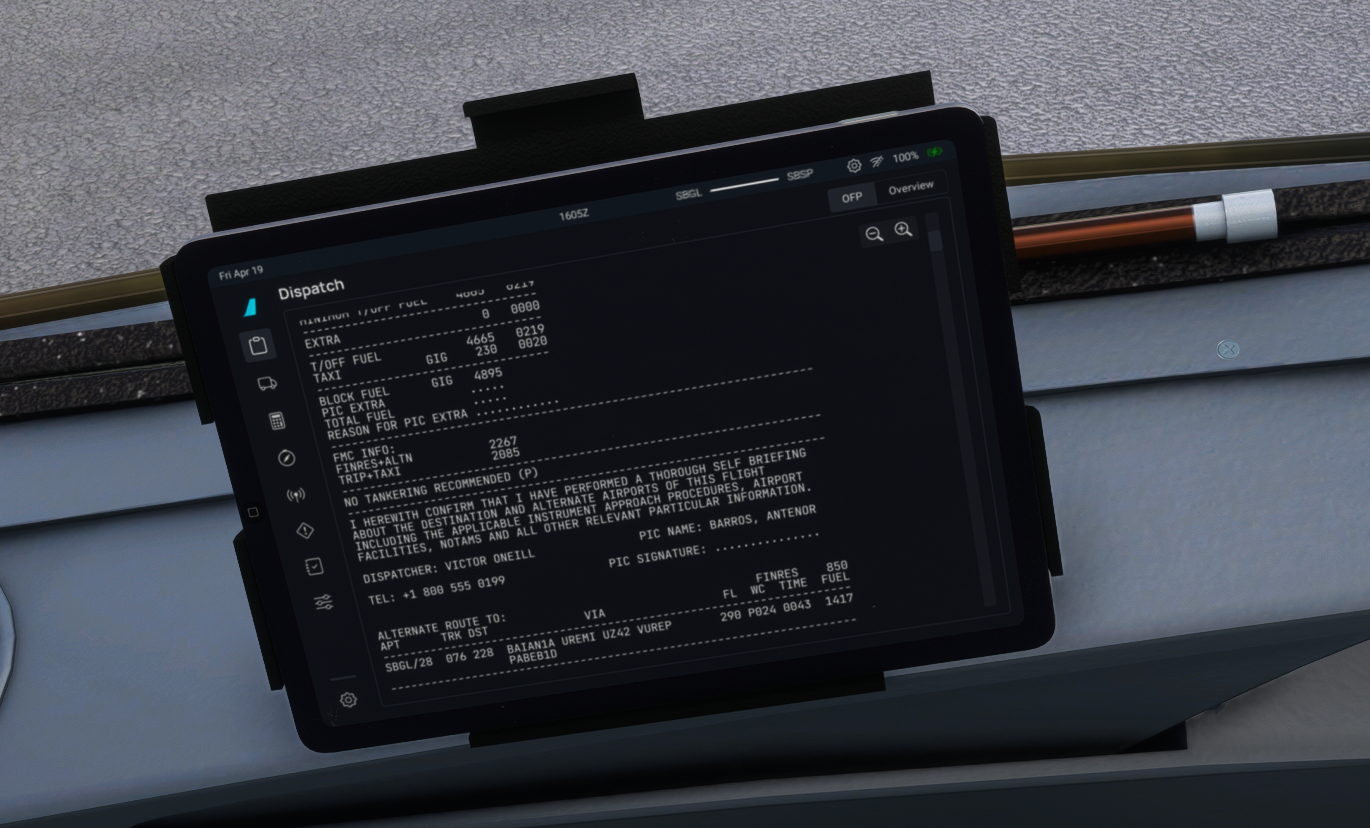
\includegraphics[width=0.47\linewidth]{img/efb-a320.png} }}%
    \qquad
    \subfloat[\centering Interface de um EFB real \cite{wired-efb}]{{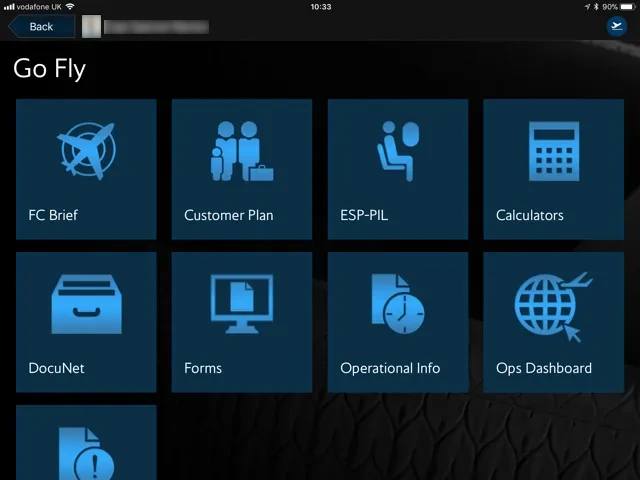
\includegraphics[width=0.45\linewidth]{img/real-flight-bag.png} }}%
    \subfloat[\centering EFB real em um Cessna Caravan]{{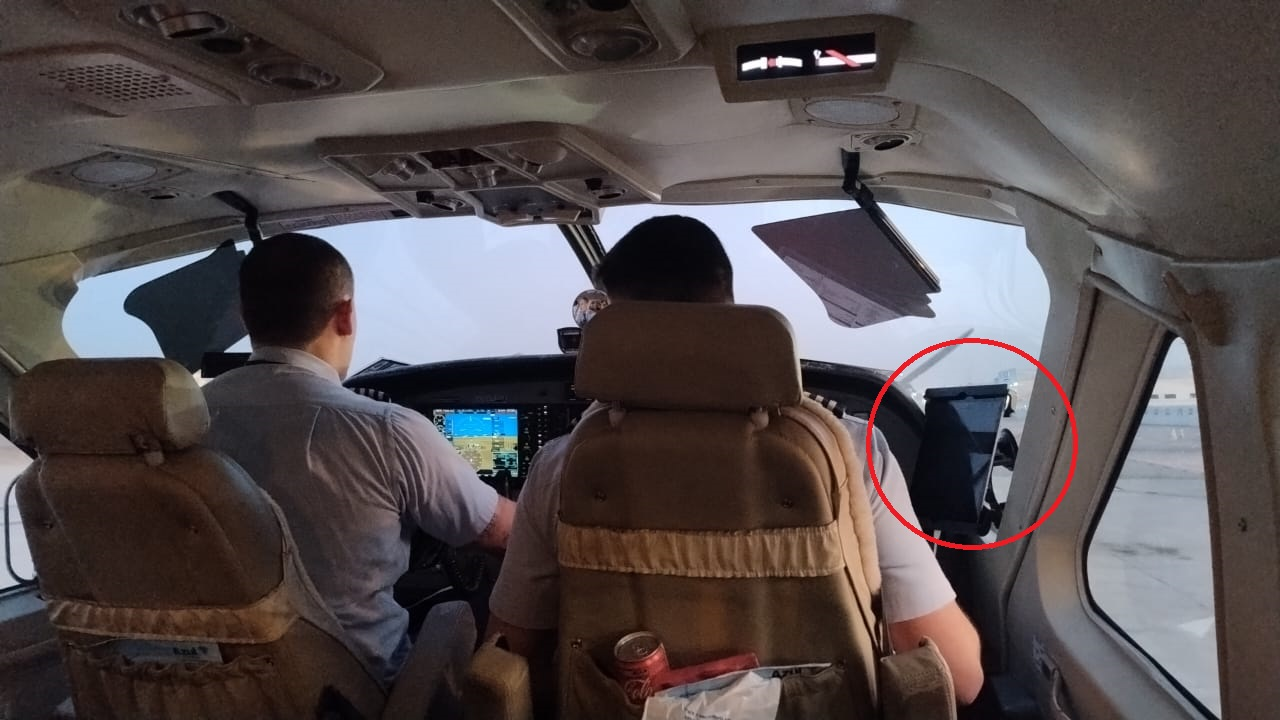
\includegraphics[width=0.6\linewidth]{img/efb-real.jpg} }}%

    \caption{Exemplos de Electronic Flight Bag (EFB)}
    
    \label{fig:example}%
\end{figure}

Uma das informações importantes para a realização de um voo é o METAR. Trata-se 
de uma string codificada com as condições meteorológicas atuais de um aeródromo. 
Todos os pilotos aprendem a ler um METAR.

Contudo, o METAR do aeródromo não se encontra disponível no EFB. É possível usar
 o computador de bordo da aeronave (FMC) e realizar um "WX Request" para conseguir 
 esta informação. Também, é 
 possível sintonizar na frequência do ATIS, mas isto só funcionará se o avião
 estiver perto do aeródromo.

O que muitos usuários de simuladores de voo fazem é acessar o AISWEB 
(\url{https://aisweb.decea.mil.br/}), sistema oficial brasileiro de informações
aeronáuticas. 

\begin{figure}[ht]
    \begin{center}
    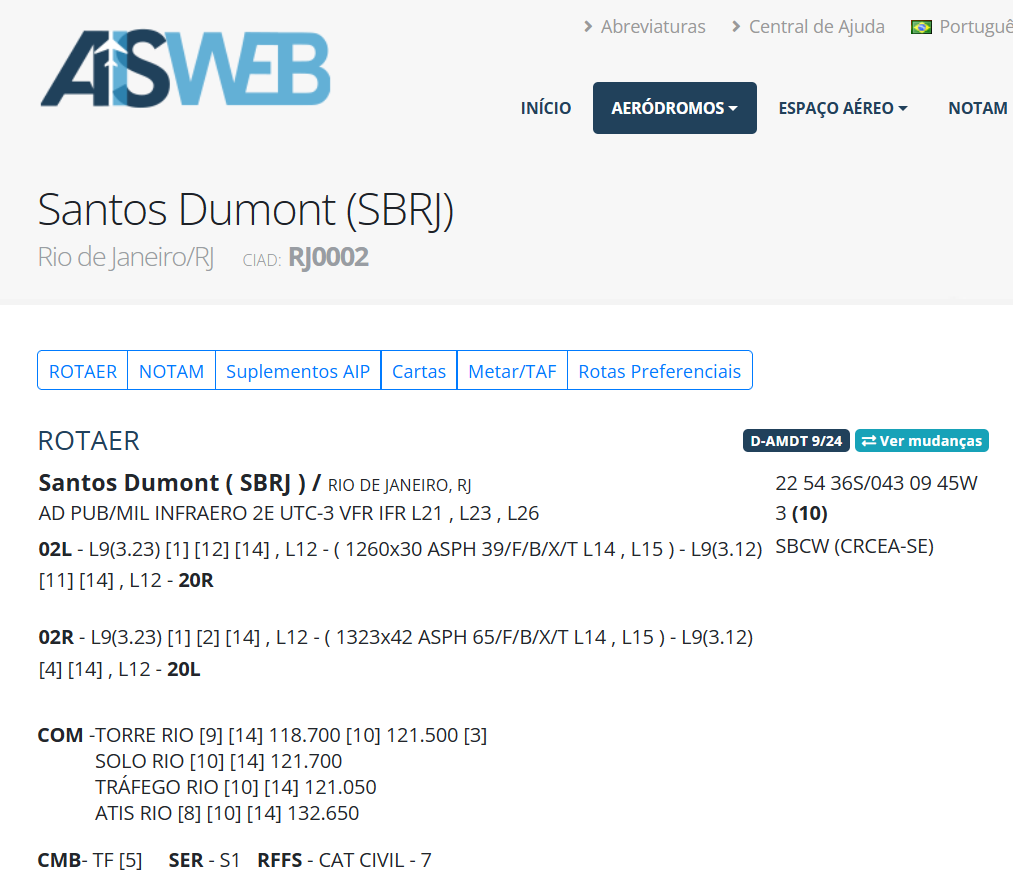
\includegraphics[width=350pt]{img/aisweb.png}
    \caption{AISWEB com informações de pista, frequências de comunicação e navegação para o Santos Dumont}
    \label{fig:aisweb}
    \end{center}
\end{figure}

É um site extremamente completo e usado em operações reais, mas para o usuário 
iniciante seria de valia uma interface mais simples. O AISWEB exibe o METAR no 
aeroporto, mas não explica para o que cada campo serve.

\begin{figure}[ht]
    \begin{center}
    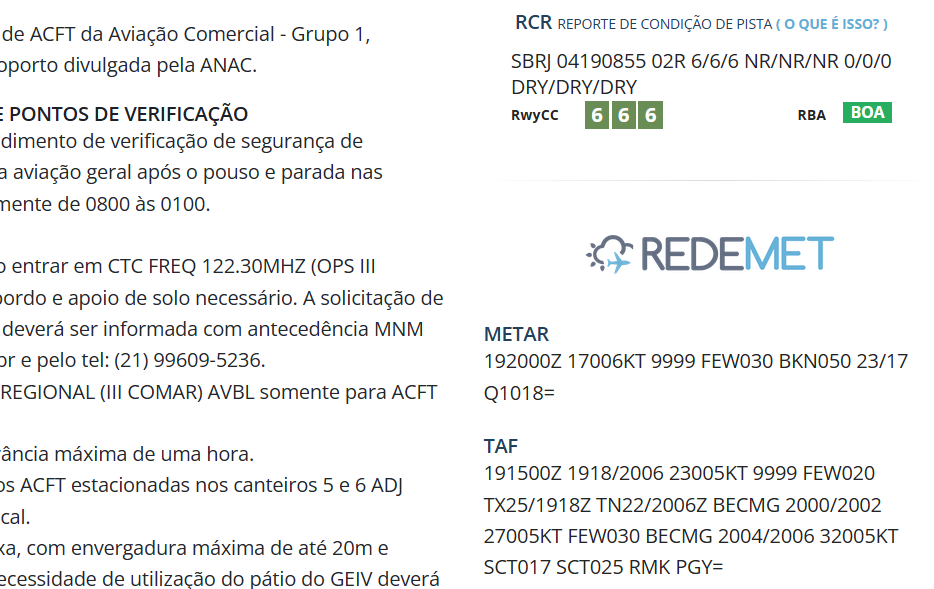
\includegraphics[width=200pt]{img/metar-aisweb.png}
    \caption{METAR do Santos Dumont no AISWEB}
    \label{fig:aisweb}
    \end{center}
\end{figure}

O site METAR-TAF (\url{https://metar-taf.com/}) é o \textit{decoder} mais conhecido. 
Possui
uma interface gráfica bem construída e muito fácil de entender, mas não possui a
lista de frequência dos aeroportos e de radionavegação. Como o nome deste sugere,
também é disponibilizado o TAF que é parecido com o METAR, mas o TAF é uma 
previsão das condições.

\begin{figure}[ht]
    \begin{center}
    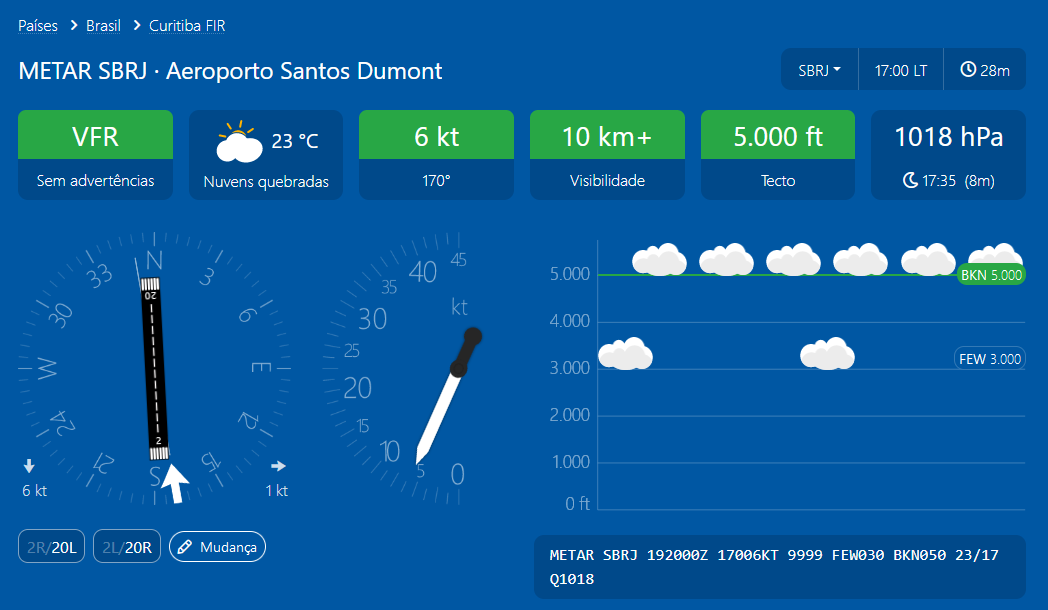
\includegraphics[width=400pt]{img/ui-metar-taf.png}
    \caption{Interface gráfica do METAR-TAF}
    \label{fig:metar-taf}
    \end{center}
\end{figure}

  % Revisão OK 26/09
\chapter{A Proposta}
A ideia do trabalho é unir as funcionalidades do METAR-TAF com o AISWEB em uma 
aplicação web que o usuário, mesmo que leigo em aviação, consiga usar sem 
dificuldades.

Pelo fato da aviação necessitar ser um ambiente seguro e bastante regulado, considerando
que meu projeto é apenas um protótipo, prefiro restringir o caso de uso apenas
para jogadores de simuladores de voo que desejam que a simulação seja parecida
com o real. As páginas terão um aviso \textbf{"APENAS PARA USO EM SIMULADOR"}.

Dito isto, o sistema possui backend escrito na linguagem Python, fazendo uso da 
framework FastAPI. Até a entrega do Projeto I, o backend era feito com Flask. 
A escolha foi feita pela minha familiaridade com a framework. Porém, depois, 
descobri a framework FastAPI no meu trabalho. Normalmente, ela não é usada para 
fullstack, mas sim para fazer APIs REST, que retornam JSON na resposta de uma 
requisição. Um frontend feito em alguma framework de JavaScript faria a requisição
 e atualizaria a página a partir dos dados recebidos.

Contudo, é possível retornar qualquer tipo de dado no FastAPI, inclusive páginas 
HTML. Como prefiro fazer a renderização de páginas no lado do servidor, continuei
usando a funcionalidade de templates do Jinja2.

A substituição da framework deu-se pelos seguintes motivos:

\begin{itemize}
\item Projeto mais maduro, continuamente mantido;
\item Documentação bem mais detalhada do que a do Flask, com vários tutoriais sobre assuntos comumente usados, como autenticação e validação de dados;
\item Pensado para validação de dados, se integra muito bem ao Pydantic;
\item Servidor embutido (Uvicorn) extremamente fácil de configurar e suficiente para produção \cite{fast-api-prod}.
No Flask é necessário configurar alguns parâmetros para o Guinicorn via o arquivo "gunicorn\_config.py";
\item Assíncrono, permitindo o uso junto com bibliotecas que utilizam asyncio;
No Flask, para paralelismo, é necessário usar uma biblioteca como o Gevent.
\end{itemize}

No segundo semestre de 2023 comecei a fazer este projeto para uso próprio.
O código está disponível em \url{https://github.com/antenor-z/aero}. Atualmente o
projeto funciona, mas a arquitetura foi feita sem muito planejamento, as
informações do aeroporto fazem parte do código.

O usuário tem acesso a informações de frequência da torre, solo, tráfego, rampa
e operações, bem como das frequências e dados para VOR (um sistema de radionavegação
por antenas no solo), ILS (sistema de pouso por instrumentos) e informações de 
pista. Neste trabalho quero, armazenar estas em um banco de dados relacional com 
uma arquitetura bem planejada. Farei testes de desempenho simulando uma alta taxa 
de acesso.

Os aeródromos podem, ao longo do tempo, mudarem alguma frequência e outras
informações, como o número da pista, que muda a depender da variação do norte 
magnético, uma ampliação da pista faz a informação de comprimento precisar ser 
alterada...

O código precisava ser alterado para atualizar estas informações. Será implementado
 um sistema administrativo no site, com uma autenticação por senha e TOTP, para 
 que seja possível mudar qualquer informação no banco mesmo por pessoas que não 
 saibam programar.

Esta parte administrativa, possui controle de permissões. Ao criar uma conta, é
 informado quais aeroportos esta conta pode alterar. Também posso dizer que esta é
  uma conta "super" que pode alterar todos os aeroportos e também criar e apagar 
 aeroportos.

  \chapter{Cronograma}

Para ter uma direção do projeto e medição da evolução, ele foi dividido 
em várias tarefas com início e duração esquematizados abaixo.

O que está em laranja são grupos de tarefas, em preto são as tarefas em si, as células com fundo 
em azul são a(s) semana(s) planejadas para realizar cada tarefa. O símbolo de losango mostra 
quando a tarefa foi de fato feita.

Em vermelho, temos tarefas que não estavam no planejamento.

\section{Cronograma do Projeto Final I}

\begin{figure}[ht]
    \begin{center}
    \includesvg[width=\linewidth]{img/cronograma.svg}
    \caption{Cronograma}
    \label{fig:cronograma-planejado}
    \end{center}
\end{figure}

Os dias 29/05 e 26/06 são milestones onde ocorrem as entregas.

\begin{table}[h]
    \centering
    \caption{Milestones}
    \begin{tabular}{|c|l|}
        \hline
        \textbf{Data} & \textbf{Milestone} \\
        \hline
        29/05 & Entrega da proposta de Projeto Final I \\
        26/06 & Entrega do relatório de Projeto Final I \\
        \hline
    \end{tabular}
\end{table}

Por ter sido meu primeiro grande projeto autogerido, tive um pouco de dificuldade em estimar o tempo real 
de implementação de cada tarefa. Portanto, há uma grande diferença entre quando uma tarefa foi estimada 
para ser feita e quando ela realmente o foi.

As seguintes tarefas são propostas para a segunda parte do projeto.

\begin{itemize}
    \item Usuários autenticados alterarem informações de um aeroporto;
    \item Cálculo da pista ativa a partir da direção do vento;
    \item Cálculo do perfil de descida;
    \item Consulta de dados históricos do METAR;
    \item Obtenção de estatísticas históricas para um aeroporto.
\end{itemize}

\section{Cronograma do Projeto Final II}

\begin{figure}[ht]
    \begin{center}
    \includesvg[width=\linewidth]{img/cronograma2.svg}
    \caption{Cronograma 2}
    \label{fig:cronograma-planejado}
    \end{center}
\end{figure}

\begin{table}[h]
    \centering
    \caption{Milestones}
    \begin{tabular}{|c|l|}
        \hline
        \textbf{Data} & \textbf{Milestone} \\
        \hline
        06/09 & Entrega do formulário de Projeto Final II \\
        01/11 & Entrega da proposta de Projeto Final II \\
        29/11 & Entrega do relatório de Projeto Final II \\
        \hline
    \end{tabular}
\end{table}
  % Revisão OK 09/10
\chapter{Decodificação do METAR}

O METAR é um protocolo de transmissão de dados meteorológicos de um aeroporto ou 
aeródromo \cite{metar-what}. Não se trata de uma previsão do tempo, mas sim de uma visualização atual. 
Para previsões existe o TAF que será explorado no próximo capítulo.
O METAR é formado por itens separados por espaço. Cada item corresponde a uma 
unidade mínima de informação meteorológica. Com os dados de sensores instalados 
no aeródromo \cite{metar-weather-gov}, a cada hora é publicado um novo METAR que
é válido para aquela hora. Em casos excepcionais, quando as condições de tempo 
estiverem mudando repentinamente, um METAR pode ser atualizado a cada meia hora
 \cite{METAR-speci} ou menos, o autor já viu o METAR do aeroporto do Galeão sendo atualizado
 na hora cheia e depois no minuto 16. Nas próximas seções, será apresentado um 
 exemplo de METAR e sua decodificação bem como uma explicação do algoritmo.

\section{Exemplo}
O METAR no aeroporto de Fortaleza (Pinto Martins)\cite{METAR-sbfz}, no dia 17 de 
abril de 2024 às 10:54 foi

\texttt{SBFZ 171300Z 15010KT 9999 BKN019 SCT025 FEW030TCU BKN100 30/25 Q1011}.

"SBFZ" se refere ao código ICAO (\textit{International Civil Aviation Organization}) do 
aeroporto, não confundir com o código IATA (\textit{International Air Transport Association}) 
que é formado por três letras. O aeroporto Pinto Martins possui o código IATA FOR, 
o Santos Dumont SDU e o Galeão GIG. O público leigo parece conhecer mais este 
código, mas na aviação costuma-se usar mais o código ICAO, pois \textit{todos} os 
aeródromos possuem um, enquanto o IATA só é presente em aeroportos onde há 
processamento de bagagem \cite{iata-codes} \cite{icao-codes}.

\begin{itemize}
\item \textbf{171300Z} significa que este METAR se refere ao dia 17 às 13 horas e zero 
minuto zulu. Horário zulu é simplesmente o fuso horário da longitude de zero grau, 
chamado de hora UTC ou Coordinated Universal Time \cite{UTC}. Para que não haja 
confusão com fusos horários, a aviação usa o horário UTC. Em tempo
estável, este 
METAR será válido até às 13:59, quando será substituído pelo METAR iniciando com 
"SBFZ 171400Z". Pode haver alteração antes em caso de mudança repentina de condições 
atmosféricas.

Note-se que a seguinte expressão regular com três grupos de captura consegue extrair 
o dia, a hora e o minuto:

\begin{verbatim}
([0-9]{2})([0-9]{2})([0-9]{2})Z
\end{verbatim}

Com o METAR supracitado, os grupos de captura serão:

\begin{itemize}
\item Grupo 1 (dia): 17
\item Grupo 2 (hora): 13
\item Grupo 3 (minuto): 00
\end{itemize}

\item \textbf{15010KT} se refere à velocidade e direção do vento. Os três primeiros 
algarismos informam a direção na bússola, em graus, de onde o vento sopra, e os 
últimos dois algarismos informam a velocidade do vento em nós (milhas náuticas por hora). 
Neste caso, o vento vem da direção 150 graus com velocidade de dez nós. Com a 
expressão abaixo extraímos essas duas informações:

\begin{verbatim}
([0-9]{3})([0-9]{2})KT
\end{verbatim}

A informação de vento pode também conter a letra G (gust) para rajadas e a letra 
V (variable) em um item separado para o caso de haver variação de direção. Por 
exemplo, um METAR com os itens \texttt{10016G21KT 080V120} informa que há rajadas 
de até 21 kt e a direção do vento pode variar de 80 a 120 graus. Existem outros 
aeroportos que podem usar outras unidades para a velocidade do vento, mas no 
Brasil só é usado nós (kt). Para obter essas informações usamos o regex 
\verb|([0-9]{3})([0-9]{2})G([0-9]{2})KT| e \verb|([0-9]{3})V([0-9]{3})|.

\item \textbf{9999} significa visibilidade ilimitada (maior ou igual a 10 km). Se fosse 
6000, a visibilidade seria de 
6 km. Por ser sempre quatro algarismos, o regex \verb|([0-9]{4})| consegue capturar 
essa informação.

\item \textbf{30/25} Temperatura 30°C e ponto de orvalho 25°C. Caso a temperatura seja 
negativa, a letra M é adicionada antes do número. M2/M5 significa temperatura 
-2°C e ponto de orvalho -5°C \cite{METAR-help}. O regex usado é

\begin{verbatim}
(M?[0-9]{2})/(M?[0-9]{2})
\end{verbatim}

Observe o M opcional. É necessário depois fazer a substituição do M para o sinal
de menos.

\item \textbf{Q1011} O altímetro do avião deve ser ajustado para 1012 hectopascal. 
Também pode ser usada a unidade polegadas de mercúrio (mmHg), mas no Brasil esta 
não é usada no METAR. O regex é\verb|(Q[0-9]{4})|

\item \textbf{SCT025} Nuvens espalhadas (3/8 a 4/8 do céu com nuvens) em 2500 pés de 
altitude. 025 se refere ao nível de voo (Flight Level), que é a altitude acima 
do nível médio do mar com divisão exata por 100.

\item \textbf{FEW030TCU} Poucas nuvens (1/8 a 2/8 do céu com nuvens) em 3000 pés de 
altitude. O sufixo TCU significa que há nuvens convectivas significativas \cite{decea-mil}.

\item \textbf{BKN100} Nuvens broken (5/8 a 7/8 do céu com nuvens) em 10000 pés de altitude.

Existe também o tipo OVC (overcast) que se refere a totalmente encoberto. O regex 
usado é \verb|([A-Z]{3})([0-9]{3})(TCU)?|. O primeiro grupo de captura é comparado 
com "FEW", "BKN", "SCT" e "OVC".

\end{itemize}

\section{Algoritmo}

O objetivo do módulo de decoder é dar uma explicação automática semelhante a esta 
para qualquer tipo de METAR de aeroportos no Brasil. O módulo usa várias expressões 
regulares para decodificar uma grande quantidade de informações, porém não é exaustivo; 
foi dada preferência a fenômenos que podem ocorrer no Brasil \cite{decea-mil}.

O algoritmo deve separar a string do METAR pelo caractere de espaço. Para cada 
item separado, cada expressão regular é testada, não é garantida uma ordem dos itens.
 Caso uma combinação ocorra, os grupos de captura são interpolados em uma string 
 que explica aquele item. 

\section{Exemplo}

Sendo "\$1" o primeiro grupo de captura, "\$2" o segundo e "\$3" o terceiro, o item "27008G16KT", 
por exemplo é comparado com todas as expressões regex e ocorre o match com apenas a seguinte:

\begin{verbatim}
  ([0-9]\{3\})([0-9]\{2\})G([0-9]\{2\})KT
\end{verbatim}

que é mapeada para a frase

\begin{verbatim}
  Vento $1° com $2 nós e rajadas de até $3 nós
\end{verbatim}

com os grupos de captura do regex supracitado. Então, será gerada uma tupla
\texttt{(27008G16KT, Vento 270° com 8 nós e rajadas de até 16 nós)}. O retorno do 
algoritmo será uma lista de tuplas enviada à ferramenta de templating
de página Jinja.

A seguir um exemplo para esta lista de tuplas:

\lstinputlisting[label=rett:metar, language=Python]{code/metar.json}

E como é mostrado na página:

\begin{figure}[ht]
  \begin{center}
  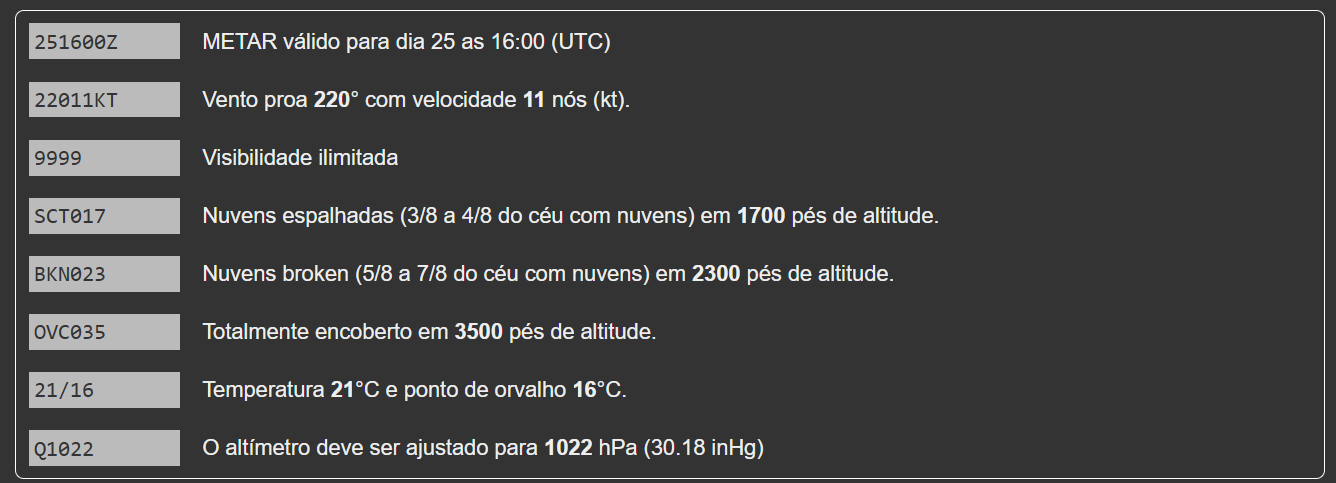
\includegraphics[width=400pt]{img/metar-sbgl.png}
  \caption{METAR do aeroporto do Galeão dia 30 de agosto de 2024}
  \label{fig:metar-30-08}
  \end{center}
\end{figure}

  % \chapter{Decodificação do METAR}
\section{Introdução}
Primeiramente em aviação falamos de duas velocidades: a velocidade do avião
 em relação a um ponto fixo no solo é a velocidade de solo (ground speed).
Com ela podemos calcular quanto tempo uma viagem demora. Mas, para efeitos de 
sustentação do avião e o que importa é a velocidade em relação ao ar (air speed). 

É importante saber a direção do vento para operações de decolagem e pouso,
pois o vento pode ajudar ou atrapalhar nestas fases críticas de voo.
O melhor cenário possível é vento vindo de frente (vento de proa) pois
será necessário menos velocidade em relação ao solo para decolagem ou 
pouso.

A velocidade do avião em relação do solo no caso do vetor vento 
paralelo ao vetor velocidade será:

\begin{align}
    V_{solo} = V_{ar} + V_{vento} \\
    V_{ar} = V_{solo} - V_{vento}
\end{align}

Sendo $V_{aviao}$ definido com sempre positivo, se o vento está 
contra o avião, o sinal de $V_{vento}$ do vento
será negativo, portanto a velociade em relação ao ar fica maior para
uma mesma velociade com o solo.

No caso oposto, com o vento de cauda, o avião precisa manter uma
velocidade em relação ao solo maior para compensar. Para o 
pouso será necessária mais distância para a parada da aeronave.
Já para a decolagem, o avião terá que usar mais pista até que
consiga levantar voo.

Contudo, normalmente o vento nunca estará perfeitamente paralelo
com a aeronave: é preciso calcular a componente do vetor vento 
paralela e perpendicular à aeronave.

Sendo V o vetor do vento, $\theta$ o menor ângulo entre o vetor 
do vento e o vetor com direção da proa da aeronave.


\begin{equation}
V = (V_x, V_y)
V_paralelo = V * cos(\theta)
V_perpendicular = V * sen(\theta)
\end{equation}


  \chapter{Modelo de Dados}

Nesta seção, vamos será explicado o modelo de dados desenvolvido para o projeto, abordando sua estrutura 
lógica e os componentes principais. O objetivo deste modelo é garantir flexibilidade para futuras alterações e 
manutenções, proporcionando uma base sólida e expansível para o aero.

\section{Modelo Lógico}

O modelo de dados foi feito de forma que futuras alterações
possam ser absorvidas facilmente. Abaixo está o diagrama entidade-relacionamento no qual
o nome no topo do retângulo identifica o nome da tabela. A lista abaixo mostra
as colunas dessas tabelas, a sigla PK denota \textit{chave primária} e FK \textit{chave estrangeira}.

Uma relação é denotada pelas setas ligando duas tabelas. A cardinalidade da relação é indicada
pelos números entre parênteses. 

Para a relação \texttt{Aerodrome-ILS}, temos (1, 1) para (0, n), significando que um aeródromo pode
ter zero ou mais frequências de ILS e esta só pode ser de um único aeródromo.

Já na relação \texttt{Aerodrome} com \texttt{Runway}, um aeródromo deve ter \texttt{uma ou mais} pistas.


\begin{figure}[ht]
    \begin{center}
    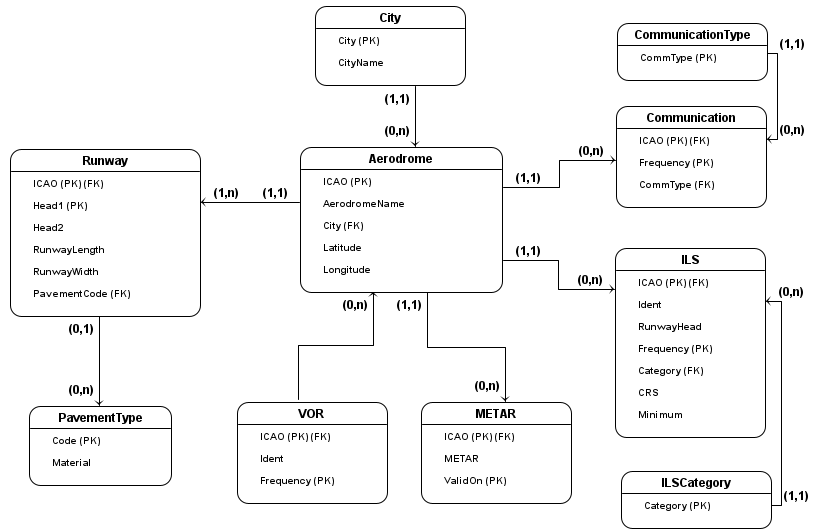
\includegraphics[width=400pt]{img/ERAero.png}
    \caption{Diagrama E/R}
    \label{fig:diagrama-er}
    \end{center}
\end{figure}

Note que as tabelas "CommunicationType", "ILSCategory" e "PavementType" poderiam ser substituídas
por colunas enum nas tabelas "Communication", "ILS" e "Runway", porém a manutenção seria difícil
\cite{table-enum},
pois teríamos que alterar a estrutura das tabelas (possivelmente tirando o sistema do ar) caso 
fosse necessário adicionar um tipo novo
de comunicação, por exemplo. Fazendo com uma tabela externa é necessário apenas adicionar uma nova
linha.

\section{Tabelas}

\begin{longtable}{|p{3cm}|p{6.6cm}|p{3cm}|}
    \caption{City} \\
    \hline
    \textbf{Nome} & \textbf{Descrição} & \textbf{Tipo} \\ \hline
    \endfirsthead
    \multicolumn{3}{c}%
    {{\tablename\ \thetable{} -- Continuação da página anterior}} \\
    \hline
    \textbf{Nome} & \textbf{Descrição} & \textbf{Tipo} \\ \hline
    \endhead
    \hline \multicolumn{3}{|r|}{{Continua na próxima página}} \\ \hline
    \endfoot
    \hline
    \endlastfoot
        City (PK)
        & Código do IBGE \cite{IBGE-cidade} da cidade
        & INTEGER
        \\ \hline
        CityName
        & Nome da cidade escrito em Português com a primeira letra maiúscula
        & VARCHAR (50)
        \\ \hline
\end{longtable}


\begin{longtable}{|p{3cm}|p{6.6cm}|p{3cm}|}
    \caption{Aerodrome} \\
    \hline
    \textbf{Nome}       & \textbf{Descrição} & \textbf{Tipo}  \\ \hline
    \endfirsthead
    \multicolumn{3}{c}%
    {{\tablename\ \thetable{} -- Continuação da página anterior}} \\
    \hline
    \textbf{Nome}       & \textbf{Descrição} & \textbf{Tipo}  \\ \hline
    \endhead
    \hline \multicolumn{3}{|r|}{{Continua na próxima página}} \\ \hline
    \endfoot
    \hline
    \endlastfoot
        ICAO (PK)
        & O código ICAO do aeródromo emitido pela Organização Internacional de Aviação Civil (ICAO).
        & VARCHAR(4)
        \\ \hline

        AerodromeName
        & O nome do aeródromo conforme definido pelo AISWEB, sistema nacional de informações aeronáuticas.
        & VARCHAR(50) 
        \\ \hline

        City (FK)
        & Chave estrangeira para o código da cidade
        & INTEGER
        \\ \hline

        Latitude 
        & A latitude do aeroporto em graus no formato de graus decimais (DD, Decimal Degrees). Três dígitos para 
        representar a parte inteira e seis dígitos para a fracionária.
        & DECIMAL(9, 6)
        \\ \hline
        
        Longitude 
        & A longitude do aeroporto, seguindo o mesmo formato da latitude. 
        & DECIMAL(9, 6)
        \\ \hline
\end{longtable}

\begin{longtable}{|p{3cm}|p{6.6cm}|p{3cm}|}
    \caption{METAR} \\
    \hline
    \textbf{Nome}       & \textbf{Descrição} & \textbf{Tipo}  \\ \hline
    \endfirsthead
    \multicolumn{3}{c}%
    {{\tablename\ \thetable{} -- Continuação da página anterior}} \\
    \hline
    \textbf{Nome}       & \textbf{Descrição} & \textbf{Tipo}  \\ \hline
    \endhead
    \hline \multicolumn{3}{|r|}{{Continua na próxima página}} \\ \hline
    \endfoot
    \hline
    \endlastfoot
        Aerodrome (PK) (FK)
        & Chave estrangeira para qual aeródromo este METAR se refere
        & VARCHAR(4)
        \\ \hline

        METAR
        & O METAR em si
        & VARCHAR(100)
        \\ \hline

        ValidOn (PK)
        & Timestamp com o momento que este metar é válido. É construído a
        partir do item do metar "ddhhmmZ" em que "dd" é o dia e "hhmm" é
        a hora zulu (UTC). O mês e ano são o mês e ano atuais do sistema.
        & DATETIME

        \\ \hline
\end{longtable}


\begin{longtable}{|p{3cm}|p{6.6cm}|p{3cm}|}
    \caption{PavementType} \\
    \hline
    \textbf{Nome}       & \textbf{Descrição}                                                                                          & \textbf{Tipo} \\ \hline
    \endfirsthead
    \multicolumn{3}{c}%
    {{\tablename\ \thetable{} -- Continuação da página anterior}} \\
    \hline
    \textbf{Nome}       & \textbf{Descrição}                                                                                          & \textbf{Tipo} \\ \hline
    \endhead
    \hline \multicolumn{3}{|r|}{{Continua na próxima página}} \\ \hline
    \endfoot
    \hline
    \endlastfoot

        Code (PK)
        & O código (em Inglês) do tipo de pavimento usado. É formado por três letras maiúsculas.
        & VARCHAR(3)
        \\ \hline

        Material 
        & O nome do pavimento em Português, com a primeira letra maiúscula.
        & VARCHAR(20)
        \\ \hline


\end{longtable}

\begin{verbatim}
Exemplo de siglas:

Code    Material
ASP     Asfalto
CON     Concreto
GVL     Brita
\end{verbatim}


É importante conhecer as características dos tipos de pistas de 
pouso e decolagem, pois seu comprimento determinará a quantidade de freio 
necessária para parar uma determinada aeronave.

Se a pista for muito curta, determinados modelos de avião não poderão pousar. 
A largura da pista determina a envergadura máxima que uma aeronave pode ter 
para operar nessa pista. Se uma pista for muito estreita, uma aeronave quadrimotora 
como o Boeing 747 pode sofrer ingestão de materiais, já que os dois motores mais 
externos ficarão para fora da área da pista, sobre o gramado.

\begin{longtable}{|p{3cm}|p{6.6cm}|p{3cm}|}
    \caption{Runway} \\
    \hline
    \textbf{Nome}       & \textbf{Descrição}                                                                                          & \textbf{Tipo} \\ \hline
    \endfirsthead
    \multicolumn{3}{c}%
    {{\tablename\ \thetable{} -- Continuação da página anterior}} \\
    \hline
    \textbf{Nome}       & \textbf{Descrição}                                                                                          & \textbf{Tipo} \\ \hline
    \endhead
    \hline \multicolumn{3}{|r|}{{Continua na próxima página}} \\ \hline
    \endfoot
    \hline
    \endlastfoot

        ICAO (FK e PK) 
        & O código ICAO do aeródromo ao qual a pista está associada, utilizado como chave estrangeira 
        fazendo a ligação com a tabela 'Aerodrome'.
        & VARCHAR(4)
        \\ \hline

        Head1 (PK) 
        & Número e possível letra que identifica uma das cabeceiras da pista. Um aeroporto nunca terá
        cabeceiras repetidas, então ICAO e Head1 formam uma chave primária mínima.
        & VARCHAR(3)
        \\ \hline

        Head2 (PK) 
        & O mesmo, mas para o outra cabeceira.
        & VARCHAR(3)
        \\ \hline

        RunwayLength
        & Comprimento da pista em metros.
        & INTEGER
        \\ \hline

        RunwayWidth
        & Largura da pista em metros.
        & INTEGER
        \\ \hline

        PavementCode (FK)
        & O tipo de pavimento da pista, referenciando a tabela 'PavementType'.
        & VARCHAR(3)
        \\ \hline

\end{longtable}

Para cabeceiras paralelas, ou seja, que apontam para a mesma direção, temos:

\subsection{Pista única}

A proa em que a pista aponta, com divisão por 10 arredondada. Por exemplo, em Fortaleza,
temos uma cabeceira com curso de 126 graus, dividindo por 10 temos 12,6, arredondando
temos o número 13 da cabeceira.

\subsection{Pista dupla}

Para duas pistas paralelas, usamos L para a cabeceira da esquerda e R para a da direita.
Por exemplo, no Santos Dumont, de costas para o Pão de Açúcar, temos as cabeceiras 02L 
(na esquerda) e 02R (na direita).

\subsection{Pista tripla}

Não temos aeroportos com três pistas paralelas no Brasil, mas são usadas as letras
L, C e R. C para a pista central.


\begin{longtable}{|p{3cm}|p{6.6cm}|p{3cm}|}
    \caption{CommunicationType} \\
    \hline
    \textbf{Nome}       & \textbf{Descrição}                                                                                          & \textbf{Tipo} \\ \hline
    \endfirsthead
    \multicolumn{3}{c}%
    {{\tablename\ \thetable{} -- Continuação da página anterior}} \\
    \hline
    \textbf{Nome}       & \textbf{Descrição}                                                                                          & \textbf{Tipo} \\ \hline
    \endhead
    \hline \multicolumn{3}{|r|}{{Continua na próxima página}} \\ \hline
    \endfoot
    \hline
    \endlastfoot

        CommType (PK)
        & O tipo de comunicação, podendo ser "Torre", "Solo", "ATIS", "Tráfego" ou "Operação".
        Mais adiante outros tipos podem ser adicionados.
        & VARCHAR(10)
        \\ \hline

\end{longtable}


\begin{longtable}{|p{3cm}|p{6.6cm}|p{3cm}|}
    \caption{Communication} \\
    \hline
    \textbf{Nome}       & \textbf{Descrição}                                                                                          & \textbf{Tipo} \\ \hline
    \endfirsthead
    \multicolumn{3}{c}%
    {{\tablename\ \thetable{} -- Continuação da página anterior}} \\
    \hline
    \textbf{Nome}       & \textbf{Descrição}                                                                                          & \textbf{Tipo} \\ \hline
    \endhead
    \hline \multicolumn{3}{|r|}{{Continua na próxima página}} \\ \hline
    \endfoot
    \hline
    \endlastfoot

        ICAO (PK e FK)
        & O código ICAO do aeródromo ao qual a frequência de comunicação está associada, utilizado 
        como chave estrangeira referenciando a tabela 'Aerodrome'.
        & VARCHAR(4)
        \\ \hline

        Frequency (PK)
        & A frequência em MHz multiplicada por 1000. Já que as frequências de comunicação possuem 
        três digitos decimais, multiplicamos por mil para armazenar em inteiro de ponto fixo. 
        ICAO e frequency formam chave primária e usar um DECIMAL para uma PK, não é muito eficiente. 
        Note que uma frequência, não necessariamente é única em todo o país, para distâncias longas, 
        onde não há risco de interferência, é possível haver frequências repetidas.
        & INTEGER
        \\ \hline

        CommType (FK)
        & O tipo de comunicação, chave estrangeira para 'CommunicationType'.
        & VARCHAR(20)
        \\ \hline

\end{longtable}


Esta tabela lista as diferentes categorias de Sistema de Pouso por Instrumentos
 (Instrument Landing System).

 \begin{longtable}{|p{3cm}|p{6.6cm}|p{3cm}|}
    \caption{ILSCategory} \\
    \hline
    \textbf{Nome}       & \textbf{Descrição}                                                                                          & \textbf{Tipo} \\ \hline
    \endfirsthead
    \multicolumn{3}{c}%
    {{\tablename\ \thetable{} -- Continuação da página anterior}} \\
    \hline
    \textbf{Nome}       & \textbf{Descrição}                                                                                          & \textbf{Tipo} \\ \hline
    \endhead
    \hline \multicolumn{3}{|r|}{{Continua na próxima página}} \\ \hline
    \endfoot
    \hline
    \endlastfoot

    Category (PK)
    & A categoria de ILS, sendo "CAT I", "CAT II", "CAT IIIA", "CAT IIIB" ou
    "CAT IIIC". Será explicado melhor em "Minimus" na tabela "ILS".
    & VARCHAR(10)
    \\ \hline

\end{longtable}

\begin{longtable}{|p{3cm}|p{6.6cm}|p{3cm}|}
    \caption{ILS} \\
    \hline
    \textbf{Nome}       & \textbf{Descrição}                                                                                          & \textbf{Tipo} \\ \hline
    \endfirsthead
    \multicolumn{3}{c}%
    {{\tablename\ \thetable{} -- Continuação da página anterior}} \\
    \hline
    \textbf{Nome}       & \textbf{Descrição}                                                                                          & \textbf{Tipo} \\ \hline
    \endhead
    \hline \multicolumn{3}{|r|}{{Continua na próxima página}} \\ \hline
    \endfoot
    \hline
    \endlastfoot

    ICAO (PK e FK)
    & O código ICAO do aeródromo ao qual o sistema de pouso está associado, utilizado 
    como chave estrangeira referenciando a tabela 'Aerodrome'.
    & VARCHAR(4)
    \\ \hline

    Frequency (PK)
    & A frequência de operação do ILS em MHz, multiplicado por 10. Fazemos isso para poder usar o tipo
    INTEGER, já que um DECIMAL como chave primária não seria eficiente, como já explicado na tabela de
    comunicação.
    & INTEGER
    \\ \hline

    Ident
    & Identificação de três letras maisculas única do ILS para aquele aeródromo.
    Aparece na carta aérea do procedimento ILS.
    & VARCHAR(3)
    \\ \hline

    RunwayHead
    & Para qual pista este ILS se refere.
    & VARCHAR(3)
    \\ \hline

    Category (FK)
    & A categoria do ILS, referenciando a tabela 'ILSCategory'.
    & VARCHAR(10)
    \\ \hline

    CRS
    & A referência do curso de aproximação do ILS. É a proa final que a aeronave deve 
    manter para o correto alinhamento nesta cabeceira.
    & INTEGER
    \\ \hline

    Minimum
    & A altura mínima de decisão em pés para operação do ILS. A partir desta altura, é
    desligado o piloto automático e o resto da aproximação é feita manualmente.
    Se a altitude da aeronave ficar abaixo deste valor e ainda não for possível 
    ter visual da pista é obrigatória a arremetida.
    
    Quando maior a categoria do ILS, maior a precisão do sistema, portanto a Minimus 
    será mais baixa. Uma "CAT IIIC" (pronuncia-se cat três charlie), possui Minimus zero, 
    portanto a aeronave pode pousar de forma totalmente automática.
    & INTEGER
    \\ \hline

\end{longtable}

Esta tabela registra os sistemas de navegação VOR/DME disponíveis em um aeródromo.
Não foi incluída uma tabela para as frequências de NDB porque este sistema
está caindo em desuso.

\begin{longtable}{|p{3cm}|p{6.6cm}|p{3cm}|}
    \caption{VOR} \\
    \hline
    \textbf{Nome}       & \textbf{Descrição}                                                                                          & \textbf{Tipo} \\ \hline
    \endfirsthead
    \multicolumn{3}{c}%
    {{\tablename\ \thetable{} -- Continuação da página anterior}} \\
    \hline
    \textbf{Nome}       & \textbf{Descrição}                                                                                          & \textbf{Tipo} \\ \hline
    \endhead
    \hline \multicolumn{3}{|r|}{{Continua na próxima página}} \\ \hline
    \endfoot
    \hline
    \endlastfoot

        ICAO (PK e FK)
        & O código ICAO do aeródromo ao qual o VOR/DME está associado, utilizado como 
        chave estrangeira referenciando a tabela 'Aerodrome'.
        & VARCHAR(4)
        \\ \hline

        Frequency (PK)
        & A frequência de operação do VOR/DME em MHz multiplicada por 10.
        & INTEGER
        \\ \hline

        Ident 
        & Identificação única do VOR/DME para aquele aeródromo. Forma chave primária
        junto com ICAO.
        & VARCHAR(3)
        \\ \hline

\end{longtable}
  \chapter{Arquitetura}

\section{Introdução}
A arquitetura foi pensada para ser implementada com o Docker e Docker Compose. Cada
programa que precisa ser executado é rodado em um serviço separado. Exceto, o Guinicorn,
todos os outros serviços usaram imagens prontas do Docker Hub o que oferece mais segurança
com as atualizações constantes.

\begin{figure}[ht]
    \begin{center}
    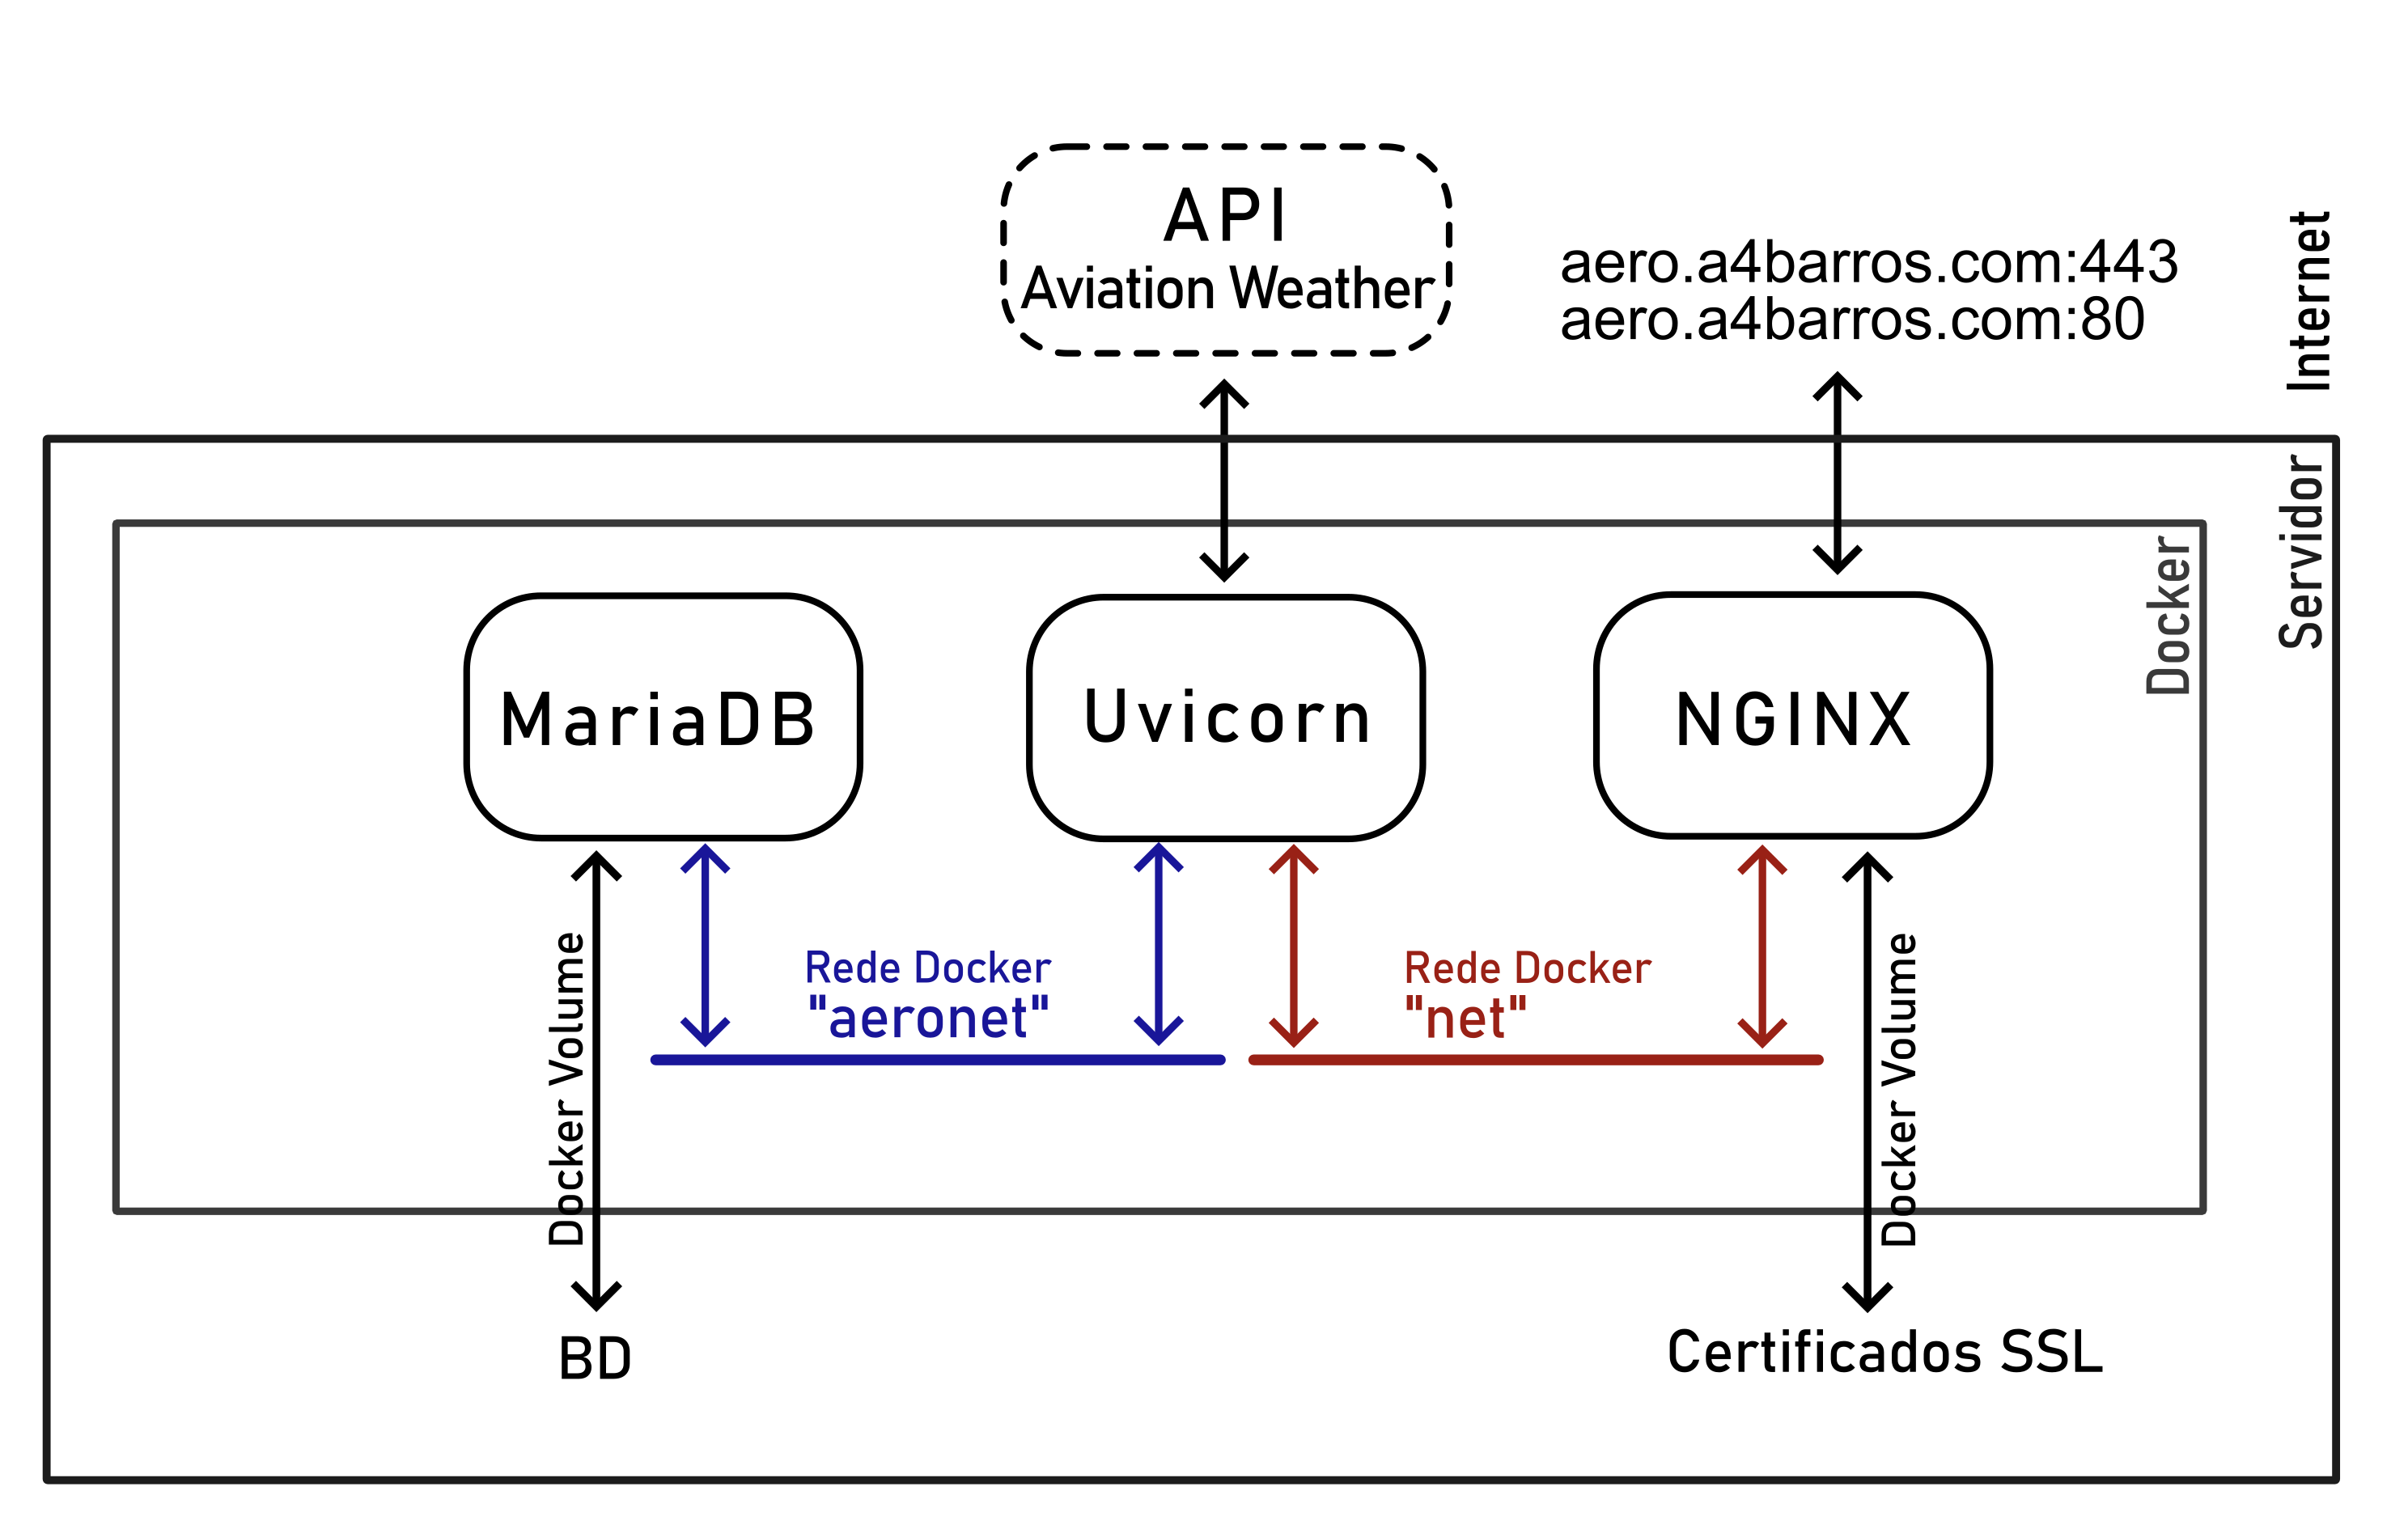
\includegraphics[width=\linewidth]{img/diagrama-arquitetura.png}
    \caption{Modelo de Arquitetura}
    \label{fig:arquitetura}
    \end{center}
\end{figure}

\section{Docker Network}
A porta 5000 do Guinicorn não estará disponível para todos os serviços. Por segurança, é usada a função de
"network". Observe no diagram que a proxy NGINX compartilha com o Guinicorn a rede "net", para o NGINX,
o Guinicorn não pode ser acessado por \texttt{localhost:5000} e sim por \texttt{http://aero:5000}, "aero"
sendo o nome do serviço no Docker Compose.

Já o banco de dados em memória Redis e o banco relacional MariaDB compartilham a rede Docker "aeronet".
Apenas eles dois e o Guinicorn possuem acesso a ela, isto é necessário para que o servidor consiga ler
e escrever valores nas tabelas do banco e ler e escrever chaves-valor no Redis. Porém o NGINX não possui
acesso aos dois bancos, por mais que os bancos tenham senhas, é uma barreira a mais contra uma invasão.

\section{Docker Secrets}

Para aumentar a segurança de acesso aos dois banco é usada a função "secrets". Nela, no Docker Compose,
você informa um arquivo de texto no host onde estará uma senha, uma senha por arquivo. No mesmo Compose,
você informa quais serviços tem acesso a cada senha, na execução dos containers, as senhas são
guardadas dentro de arquivos montados no caminho "/run/secret/algum-nome.txt" em que "algum-nome" é
o mesmo nome do arquivo que estava no host.
Tanto os bancos como o servidor Guinicorn usam este método para terem acessos às senhas dos bancos.

\section{Serviços}

\subsection{MariaDB}
Este banco de dados relacional guarda toda a informação mais ou menos fixa sobre os aerodromos
conforme explicado no capítulo de modelo de dados.

\subsection{Redis}
O Redis é um banco de acesso mais rápido por estar com as informações salvas em memória em vez
de disco rígido/SSD. Ele é um espelho do que existe no banco relacional, claro que com as devidas
modificações já que o Redis possui sistema-chave valor, não sendo relacional.

\subsection{Proxy NGINX}
Faz o HTTPS funcionar, dá suporte ao HTTP/2 e ao header HTTP keep-alive. O Guinicorn só tem suporte
ao primeiro. De qualquer caso a documentação do Guinicorn não recomenda que ele esteja diretamente
ligado a Intenet \cite{nginx-gunicorn}. Já que tenho outros projetos na mesma máquina, uso subdomínios.
Na configuração do NGINX o server block com hostname aero.a4barros.com é redirecionado para 
o endereço interno "https://aero:5000".

\section{Flask/Guinicorn}

Já que o Guinicorn é o serviço principal: o servidor onde o backend implementado em Flask roda,
fiz um Dockerfile próprio iniciando a partir de uma imagem do Alpine, devido ser lightweight.
O Python e as dependencias do projeto são instaladas automaticamente pelo Dockerfile e por
fim o arquivo de entrada \texttt{server.py} é executado usando o servidor Guinicorn. As configurações
dele ficam no arquivo \texttt{gunicorn\_config.py} é apenas configura a porta para 5000 e usa três workers.

A documentação do Guinicorn informa a seguinte fórmula para determinar a quantidade de workers. \cite{number-work}

\begin{equation} 
    \begin{split}
        N_{worker} = 2 * N_{cores} + 1 \\
        N_{worker} = 2 * 1 + 1 = 3 
    \end{split}
\end{equation}

\section{Produção}
O site se encontra no produção no endereço https://aero.a4barros.com. Ele está hospedado em uma VPS
com as seguintes características:

\begin{itemize}
    \item \textbf{CPU:} AMD EPYC 7713 (1 core disponível) @ 2GHz
    \item \textbf{RAM:} 1GB
    \item \textbf{Armazenamento:} 25GB
    \item \textbf{SO:} Ubuntu 22.04.4 LTS
\end{itemize}

\begin{figure}[ht]
    \begin{center}
    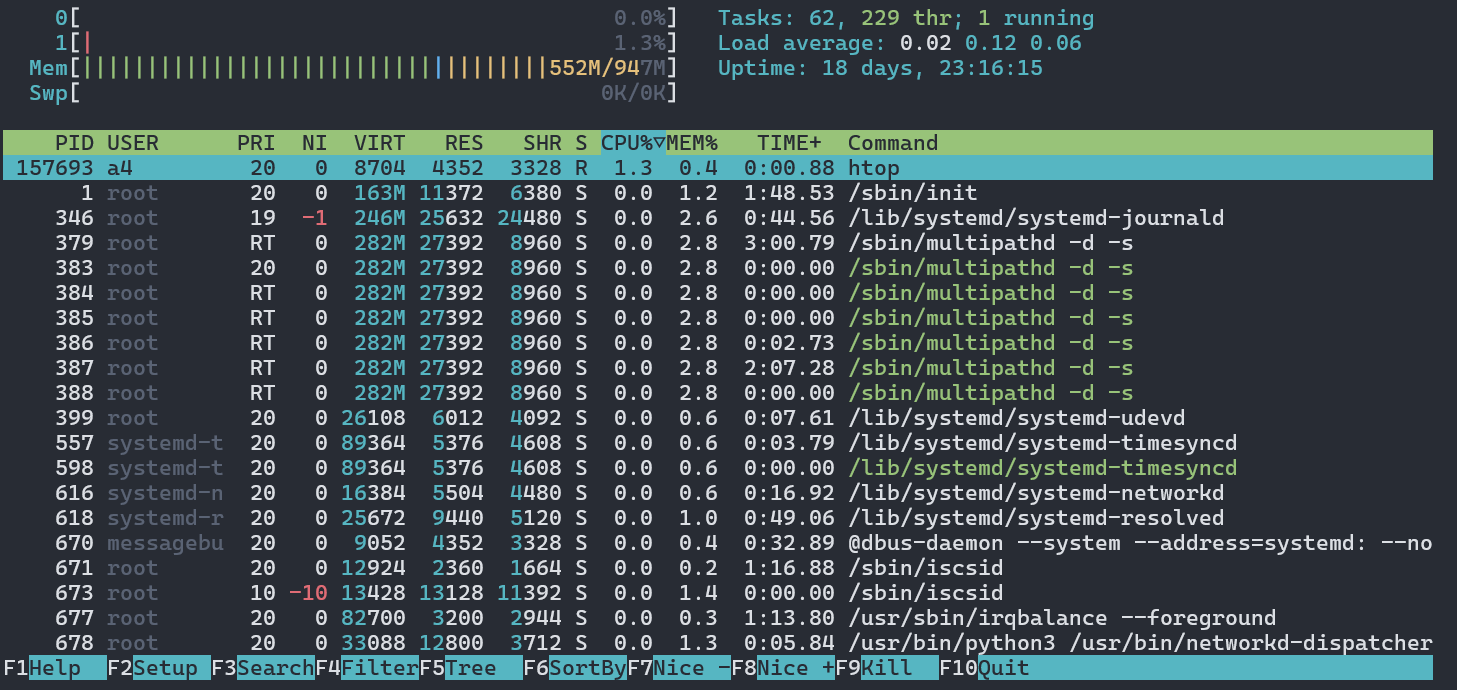
\includegraphics[width=400pt]{img/prod-idle.png}
    \caption{Uso do sistema em baixa demanda}
    \label{fig:prod-idle}
    \end{center}
\end{figure}


Mesmo com uma configuração bastante modesta, o sistema roda sete containers Docker usando 
aproximadamente metade da memória primária (RAM) em idle.

\begin{figure}[ht]
    \begin{center}
    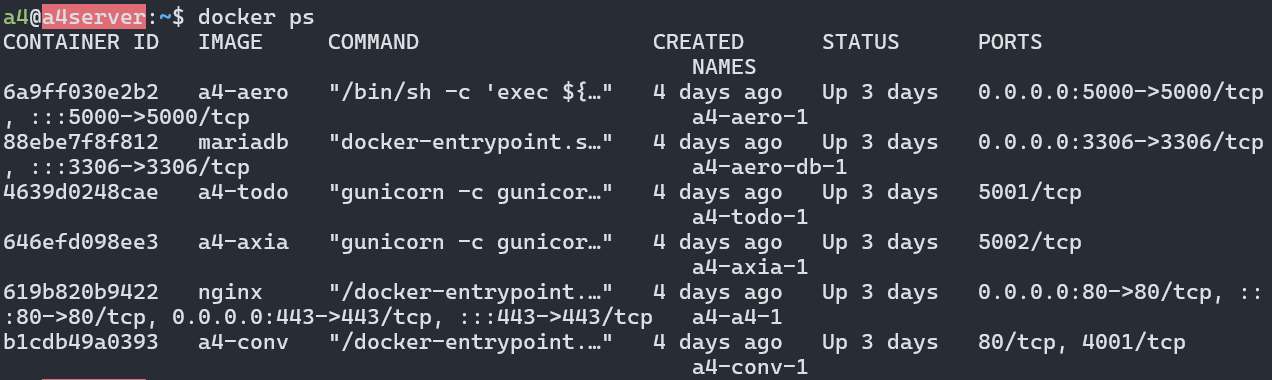
\includegraphics[width=400pt]{img/containers.png}
    \caption{Containers Docker em execução}
    \label{fig:containers}
    \end{center}
\end{figure}



  % \chapter{Front-end}

Como falado no capítulo da arquitetura, a página é gerada server-side, então o que 
é retornado para cada rota é um HTML já pronto. Acredito que, para o meu caso, é mais 
performático fazer assim do que usar páginas com Javascript que fazem requisição para uma API REST.

De todo modo, no final da execução de uma rota, um dicionário Python é gerado, algo que 
poderia ser facilmente convertido para um JSON usando a função \texttt{dumps()} da 
biblioteca \texttt{json} do próprio Python. No caso desta aplicação, este dicionário é 
enviado para o template usando a função \texttt{render\_template()} da biblioteca Jinja2, 
que recebe o nome da página HTML com o template e um número qualquer de \textit{kwargs} (argumentos nomeados) 
que podem ter qualquer tipo serializável, incluindo dicionários.

Perceba que não há problema de acoplamento fazendo deste modo, pois não há código HTML sendo 
escrito dentro do backend. Como já dito, o que é passado para o Jinja é algo equivalente a JSON.

Um página template é um arquivo HTML com \textit{placeholders} que serão substituídos pelos 
\textit{kwargs} de mesmo nome. O Jinja2 tem estruturas de repetição para que um código HTML 
possa ser repetido usando valores da lista. E, no caso de dicionários, é fácil acessar 
os valores. Neste projeto, para exibir a lista de frequência, o seguinte código é usado.

Note que é possível fazer operações e formatações simples no Jinja2. Já que a frequência 
é armazenada no banco como um inteiro de ponto fixo (como dito no capítulo de modelo de dados), 
foi criado o filtro "frequency3" para exibir o número corretamente. Um "filtro" no Jinja 
é apenas uma função que recebe e retorna
uma string. O filtro é "chamado" usando a sintaxe "\{\{variavel | funcao\}\}". Para os que tem
experiência com Linux é parecido com a ideia do operador "pipe".

\lstinputlisting[label=cod:jinja-comm,title={Template de comunicação com o Jinja},caption={Template de comunicação com o Jinja},language=HTML]{code/jinja-comm.html}

Note que caso a variável "isAdmin" seja definida, um botão de alterar a frequência aparece. Este
e outros botões de adição e edição são mostrados quando o login é feito para que o administrador
consiga editar um aeródromo.

No código do projeto, na pasta 'templates', é possível ver todos os templates usados.

\section{Minificação}

Removendo os espaços e caracteres de nova linha é possível diminuir o tamanho dos arquivos enviados
para o usuário. Após este processo, cada arquivo html, js etc fica com apenas uma linha, os menos linhas
no caso dos css, obviamente não é fácil para um humano entender, mas o navegador consegue fazer o 
parsing sem problemas. Isto é chamado de {\em minification} ou minificação. Com os arquivos
com menor tamanho, a transferência servidor para cliente é terminada mais rápido, logo a experiência
para o usuário torna-se mais agradável, já que as páginas carregam mais rápido.

Para a tabela abaixo cada tamanho em kB e cada tempo em ms se refere a média simples dos valores 
encontrados na aba "rede" das ferramentas de desenvolvedor do navegador Firefox em cinco 
carregamentos da página. A opção de desabilitar cache foi usada.

Legenda para a tabela abaixo
\begin{itemize}
\item \textbf{A:} Tamanho do arquivo sem minification
\item \textbf{B:} Tempo de carregamento deste arquivo
\item \textbf{C:} Tamanho do arquivo com minification
\item \textbf{D:} Tempo de carregamento deste arquivo
\end {itemize}

O "Tamanho" refere-se a quantidade de bytes transferidos (com compactação gzip) e não ao 
tamanho do arquivo após a compactação já que isto é feito no lado do usuário pelo navegador.

\begin{longtable}{|p{4cm}|p{2.15cm}|p{2.15cm}|p{2.15cm}|p{2.15cm}|}
    \caption{Com e Sem minification} \\
    \hline
    \textbf{Arquivo} & \textbf{A} & \textbf{B} & \textbf{C} & \textbf{D} \\ \hline
    \endfirsthead
    \multicolumn{5}{c}%
    {{\tablename\ \thetable{} -- Continuação da página anterior}} \\
    \hline
    \textbf{Arquivo} & \textbf{A} & \textbf{B} & \textbf{C} & \textbf{D} \\ \hline
    \endhead
    \hline \multicolumn{5}{|r|}{{Continua na próxima página}} \\ \hline
    \endfoot
    \hline
    \endlastfoot
        SBGR
        & 5,88 kB
        & 130 ms
        & 4,93 kB
        & 57 ms
        \\ \hline
        style.css
        & 3,45 kB
        & 68 ms
        & 2,49 kB
        & 33 ms
        \\ \hline
        tooltip.css
        & 960 B
        & 67 ms
        & 831 B
        & 24 ms
        \\ \hline
        rwy.css
        & 590 B
        & 36 ms
        & 518 B
        & 38 ms
        \\ \hline
        \texttt{Total}
        & 11.35 kB
        & 363 ms
        & 9.21 kB
        & 196 ms
        \\ \hline
\end{longtable}

Fazendo

\[
\text{x\%} = \frac{x_{\text{initial}} - x_{\text{final}}}{x_{\text{initial}}} \times 100\%
\]

É possível ver uma economia de 18,9\% na quantidade de informações enviadas. E um tempo de resposta
46,0\% menor.


  % % Revisão OK 12/10
\chapter{Rotas do back-end}

A seguir são listadas e explicadas todas as rotas públicas do backend. As
rotas de administração são explicadas na seção "Interface de Administração".

\section{Rota raiz}

Página inicial, apresenta a lista de aeródromos para que o usuário escolha um. 
Internamente, por meio do ORM, é feita a seleção dos campos \texttt{AerodromeName},
\texttt{ICAO} e \texttt{City} dos aeródromos com isPublished como verdadeiro e o
 resultado é posto em uma lista de tuplas que é enviada para o template.

Para um usuário logado também são mostrados os aeródromos não publicados.

Exemplo do resultado enviado à ferramenta de template:

\lstinputlisting[label=resp:root, title={Resposta da root}, caption={Resposta da root}, language=Python]{code/resp-root.json}


\section{Rota: /info/\{ICAO\}}

Retorna informações do aerodrómo e seu metar decodificado. A seguir um exemplo
de resultado enviado ao \textit{Jinja2}.

\lstinputlisting[label=resp:root, title={Resposta da rota info}, caption={Resposta da rota info}, language=Python]{code/resp-info.json}


\section{Rota: /history/\{ICAO\}}
É uma página estática com os gráficos históricos para os doze últimos METARs.
Mais informações do capítulo "Plotagem do METAR Histórico".


\section{Rota: /taf/\{ICAO\}}
Retorna o próximo TAF válido para este aeródromo com a explicação de cada item.

Exemplo do resultado enviado à ferramenta de template para o aeroporto do Galeão.

\lstinputlisting[label=resp:root, title={Resposta da rota taf}, caption={Resposta da rota tag}, language=Python]{code/resp-taf.json}


\begin{figure}[ht]
    \begin{center}
    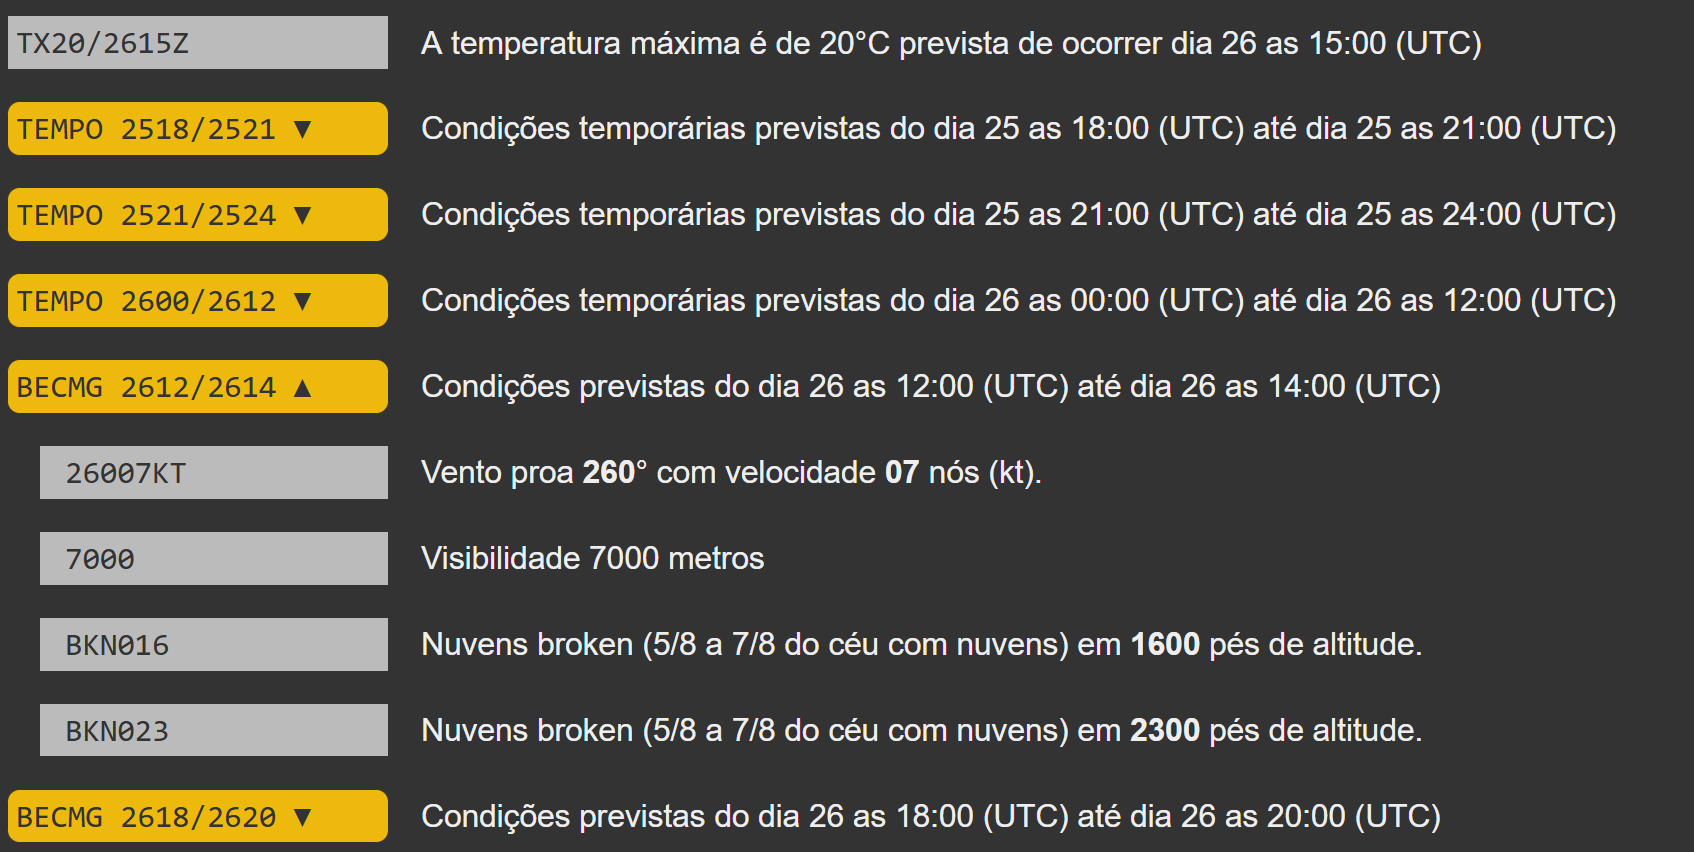
\includegraphics[width=400pt]{img/BECMG-exibido.png}
    \caption{Grupo BECMG exibido}
    \label{fig:becmg-exibido}
    \end{center}
\end{figure}

\section{Rota: /descent}

Página estática onde é possível calcular o perfil de descida. Dada a altitude
inicial, altitude final, velocidade e razão de descida (graus o pés) por minuto
é retornado a distância horizontal requerida e o tempo requerido para fazer esta
descida. O cálculo é feito apenas com JavaScript na própria página.

\section{Rota: /wind}
Dada a direção da pista, a direção do vento e velocidade do vento, é calculada
a componente paralela e perpendicular do vetor de vento em relação à aeronave.
Consulte a capítulo de front end para ver imagens da interface desta e das outras
rotas.

\section{Rota: /windcalc}
Usada pela rota anterior para calcular as componentes do vento. Para a chamada
\verb|/windcalc/?wind_dir=100&wind_speed=3&runway_head=90| a resposta será

\verb|{"cross":0.52,"head":2.95,"angle":10.0}|

Os valores retornados serão mostrados para o usuário como números e também serão
usados para modificar uma imagem SVG que mostra graficamente a influência das
componentes de vento.

\section{Rota: /wind/\{icao\}}
Parecida com a rota anterior, mas considera cada cabeceira do aeródromo selecionado
e o vento atual.




  % Revisão OK 12/10
\chapter{Conclusão}

Como conclusão, pode-se dizer que foi um projeto muito interessante de se fazer já que 
o autor tem interesse tanto da área de programação para web como a de aviação. Trata-se
de um primeiro 
projeto open-source grande e os utilizadores podem melhorar o produto mesmo sendo
leigos em programação já que na parte inferior da página principal há um e-mail 
de contato para que me sejam enviados elogios, críticas e sugestões.

Foi explorado, também, um pouco do frontend, área que que o autor não tinha tanta 
familiaridade.

Acredito que o objetivo do projeto foi alcançado. O Aero busca juntar as funcionalidades 
comumente usadas na simulação de voo em uma plataforma acessível e amigável, 
trazendo um maior nível de realismo na simulação de voo, aspecto desejado por quem leva
a simulação de voo "a sério".

Vários assuntos que não conhecia aprendi com este projeto incluindo:

\begin{itemize}
\item Fazer uma página de observabilidade
\item Fazer um teste de carga
\item Usar o \textit{Docker} Secrets para armazenar senhas ao invés do ".env"
\item Usar cache direto no NGINX para evitar que o site saia do ar em períodos 
de muitos acessos
\item Armazenar hash de senha com salt o padrão bcrypt
\item Implementar autenticação de dois fatores TOTP
\item Traduzir mensagens de erros do Pydantic para o Português para que possam 
ser mostrados para o usuário.
\end{itemize}

Acreditamos fortemente que este foi um projeto muito proveitoso devido aos 
conhecimentos de programação web que adquiridos que serão de grande valia no meu 
trabalho que é o desenvolvimento do backend de um PWA. Além disso, já que o site está público 
servirá como uma vitrine para outras potenciais oportunidades de carreira.

\section {Código completo}

O código fonte na íntegra do Aero pode ser visto acessando o seguinte link: \url{https://github.com/antenor-z/aero}

O código LaTeX que gerou este documento está disponível em: \url{https://github.com/antenor-z/aero-relatorio}

Por fim, o código apresentação de slides feita no Beamer está disponível em: \url{https://github.com/antenor-z/aero-presentation}
  
  \arial
  \bibliographystyle{abnt-num} % \bibliographystyle{abnt-alf}
  \bibliography{main} 
\end{document}
